\chapter{ExxonMobil Code Alterations}
\label{ch:appendixexxonmobil}
This \appendixname{} contains a list of modifications made to the ExxonMobil model during the testing and evaluation.

\section{1st Cell of \codefont{scratch\_pad.ipynb}}

The code was organized by creating separate folders for input and output files, facilitating easier usage and data storage. Additional modifications were made to the original source code to ensure compatibility with different operating systems, as it was previously designed exclusively for Windows and was ``Path'' sensitive.

\begin{codemodifications}

\begin{codemodification}{1}
Importing \textcode{os} library for further use.
\end{codemodification}

\begin{codemodification}{5, 11}
The lines which are from original file were commented out and replaced with new code lines.
\end{codemodification}

\begin{codemodification}{7-8, 11}
The issue with original files was that the Path/Location of the files had to be renamed for every user since the username is not same for every computer. Hence, we added new variables that will locate the current folder, the output and input files along with their directories regardless of operating system and the location of the files.
\end{codemodification}

\end{codemodifications}

\section{2nd Cell of \codefont{scratch\_pad.ipynb}}
This cell needs to be run after running the first cell if you don't have the output file from previous simulations. However, if you have the output file from previous simulations, you can skip the first cell and directly run this second cell which will save a lot of time and computational energy. The modifications were primarily made in location part. 
\begin{codemodifications}

\begin{codemodification}{1}
This line was removed since it was duplicate.
\end{codemodification}

\begin{codemodification}{5}
Importing \textcode{os} library for further use.
\end{codemodification}

\begin{codemodification}{6-9}
The original line was replaced with new lines which allow to import the data for further use since the original line of code was 'Path' sensitive.
\end{codemodification}

\end{codemodifications} 

\section{File \codefont{bitrock.py}}
The following change is related to the issue that was addressed in the final section of \chaptername~\ref{ch:exxonmobilmodel}.
A full comparison of outputs between original and modified models has been provided in \figurename~\ref{Comaprison_on_bottom}.
\begin{codemodifications}

\begin{codemodification}{29}
Originally, the variable \textcode{bit\_depth} was set to \textcode{z}. However, since \textcode{z} signifies displacement and not the actual bit depth, it does not accurately represent the true bit depth. To obtain the correct bit depth, the displacement needed to be added to the original bit depth, resulting in a list of updated bit depths for each calculation time step.
\end{codemodification}
\end{codemodifications}

The outputs obtained from the original model are presented in the left column, while those from the modified version are displayed in the right column (\figurename~\ref{Comaprison_on_bottom}). A thorough comparison is made between the two sets of outputs to observe any differences or improvements resulting from the modifications. 

To delve deeper into the on-bottom case, we conducted a model run using a specific approach, where the bit is initially raised from the bottom to simulate the off-bottom case, and then gradually brought into contact with the bottom to transition to the on-bottom case. The results clearly illustrate the effect in subsequent plots.

Upon observation, the drilling process commences at approximately 30 seconds. Initially, vibrations occur, which is typical, but as soon as the bit makes contact with the bottom at 30 seconds, both the bit and top-drive torque increase, along with WOB and DOC. Furthermore, the hole depth starts to change simultaneously with the bit depth, indicating the initiation of the drilling mode. Around 20 seconds later, the vibrations gradually diminish, indicating the presence of oscillations in the system.

\begin{figure}
  \centering
  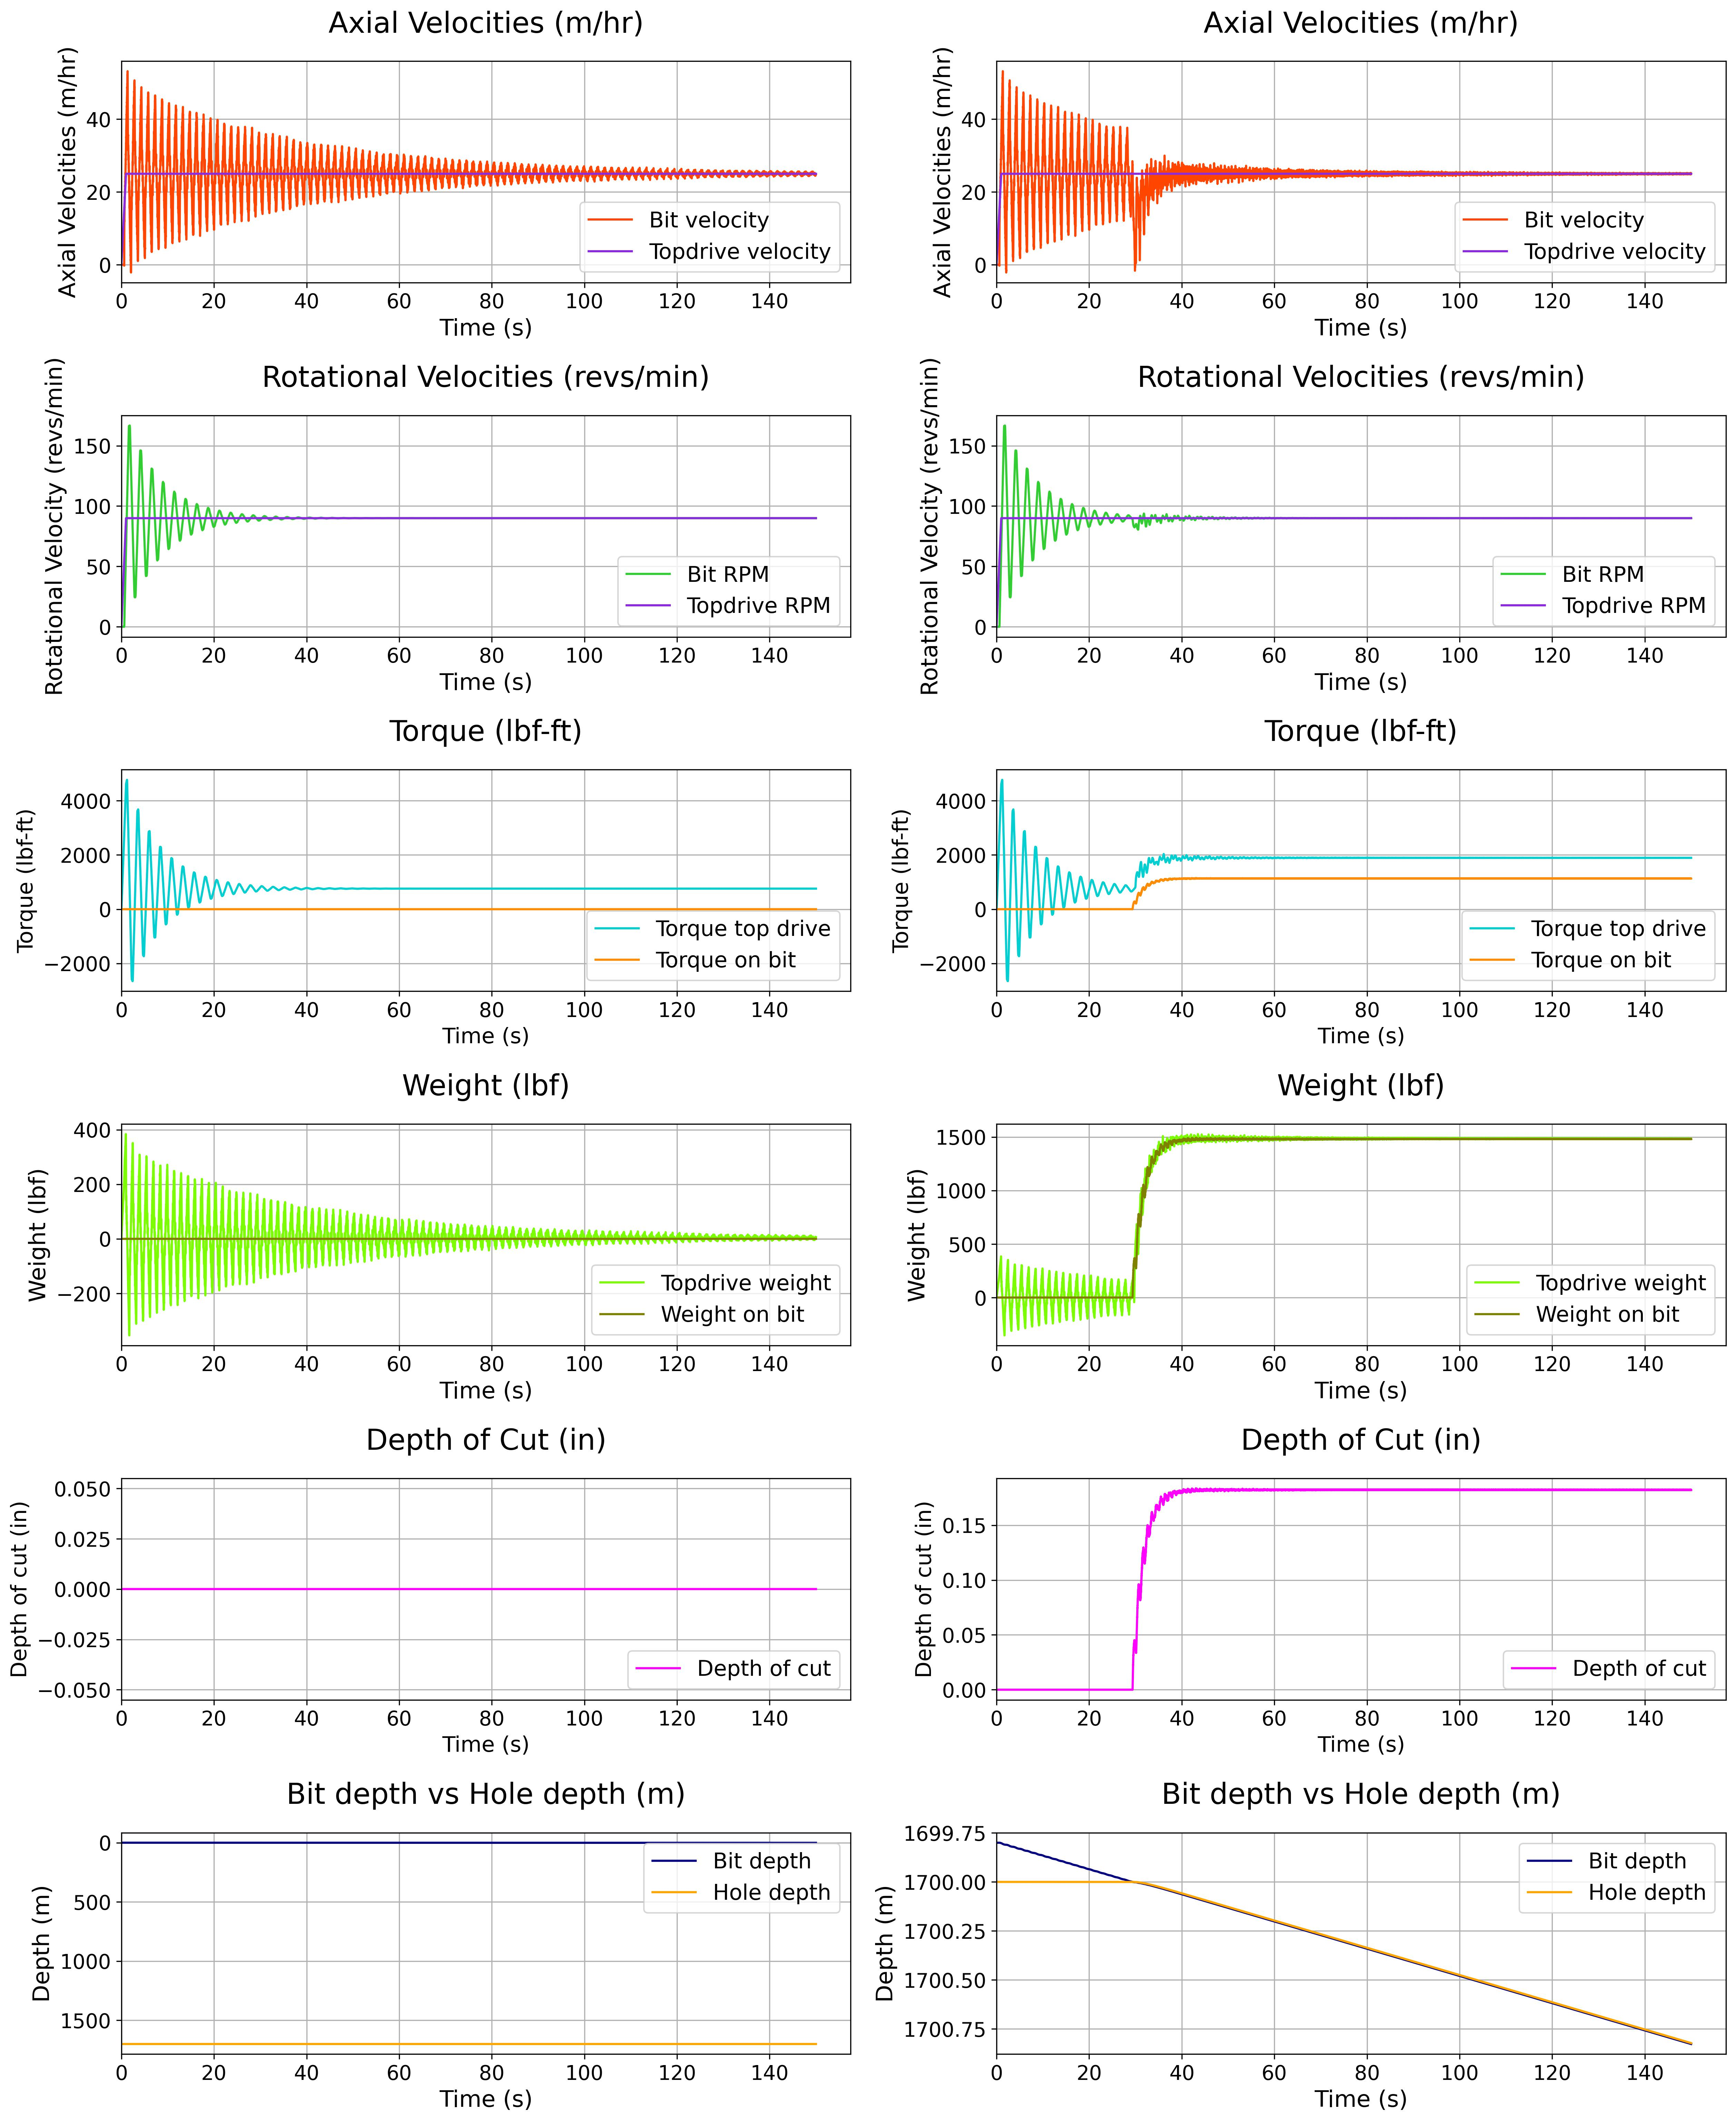
\includegraphics[width=\linewidth]{comp_on_bottom}
  \caption[Output comparison or original and modified model]{Comparison of outputs from original and modified versions of model. Figures in first and second column are the results from original code and from modified code, respectively.}\label{Comaprison_on_bottom}
\end{figure}